%%%%%%%%%%%%%%%%%%%%%%%%%%%%%%%%%%%%%%%%%%%%%%%%%%%%%%%%%%%%%%%%%%%%%%%%%%%%%
%% obtained from https://canvas.uva.nl/courses/6063/files/folder/Templates %%
%%%%%%%%%%%%%%%%%%%%%%%%%%%%%%%%%%%%%%%%%%%%%%%%%%%%%%%%%%%%%%%%%%%%%%%%%%%%%
\documentclass{uvamath}
\usepackage[english]{babel}


\usepackage{graphicx}
\graphicspath{{assets/}}
\usepackage{graphbox}
\usepackage{amssymb}
\usepackage{amsmath}
\usepackage{amsthm}
\usepackage[pdfborder={0 0 0}]{hyperref}

\usepackage{csquotes,xpatch} % Recommended by biblatex
\usepackage[
    style=numeric]{biblatex}
\addbibresource{zotero.bib}
\addbibresource{manual.bib}

\newcommand{\N}{\mathbb{N}}


\title{Local Flag Algebras: Bounding the Strong Chromatic Index} % Title of your thesis
\author[eoin.davey@student.uva.nl, 14246287]{Eoin Davey} %Your name, email and student number

\documentTitle{Master Thesis}
\program{MSc Mathematics} % MSc Mathematics / MSc Mathematical Physics / Stochastics and Financial Mathematics

\supervisorsTitle{Dr. J.R. Kang} %This is the list of supervisors for the title page, seperate with \newline

\supervisors{Dr. J.R. Kang} %This is the list of supervisors for the second page, seperate with comma

\secondexaminer{Dr. K. Guo} %This is the name of the second examiner, for the second page
\date{June 28, 2024} %This is the examination date, i.e. the date of your thesis presentation

\newtheorem{theorem}{Theorem}[chapter]
\newtheorem{lemma}{Lemma}[chapter]
\newtheorem*{knowntheorem}{Theorem}
\newtheorem{conjecture}{Conjecture}
\newtheorem*{note}{Note}
\newtheorem{definition}{Definition}[chapter]
\newtheorem*{example}{Example}

\begin{document}
\maketitle

\begin{abstract}
Scientific abstract (5-10 lines)
\end{abstract}

\tableofcontents

\chapter*{Introduction}
\addcontentsline{toc}{chapter}{Introduction}

Consider a simple\footnote{An undirected graph with no self loops and at most 1 edge between any two
vertices.} graph $G$. How many colours do you need to colour the edges such that no two edges which touch
have the same colour? What if no two edges which touch some common edge can have the same colour?
Erd\H{o}s and Nešetřil conjectured that you only need $1.25\Delta(G)^2$ colours where $\Delta(G)$ denotes the maximum degree of $G$, but
the current best proof only shows an upper bound of $1.772\Delta(G)^2$ colours (for large enough $\Delta(G)$). In this thesis
we show how we can lower this to $1.73\Delta(G)^2$ by introducing a novel framework
which is a modification of Razborov's flag algebras. We also apply this new framework
to some other problems including a bounded-degree variant of the
Erd\H{o}s's pentagon conjecture.

\section*{Strong Edge Colouring}
\addcontentsline{toc}{section}{Strong Edge Colouring}
\label{sec:intro_strong_edge_coloring}

An edge colouring of a simple graph $G$ is an assignment $c\colon E(G) \to [k]$
for some $k\in\N$. Such a colouring is \textit{proper} if no two incident\footnote{Have a vertex in common}
edges have the same colour.
An edge colouring is \textit{strong} if no two edges which share a common incident edge have
the same colour. Put differently, proper edge colouring requires edges at distance 1 to have distinct
colours and strong edge colouring extends this to distance 2.
In figure \ref{fig:proper-strong-example} we see an example of a non-proper edge colouring,
a proper (but not strong) edge colouring and a strong edge colouring of $C_5$, the cycle on $5$ vertices.

\begin{figure}[h]
    \centering
    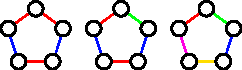
\includegraphics[scale=1.5]{proper-strong-example}
    \caption{Non-Proper, Proper \& Strong Edge Colourings}
    \label{fig:proper-strong-example}
\end{figure}

The \textit{chromatic index} of $G$, denoted $\chi'(G)$, is the minimum $k$ such that a proper edge
colouring of $G$ with $k$ colours exists. The \textit{strong chromatic index} $\chi'_s(G)$
is the corresponding minimum number of colours required for a strong edge colouring.

Vizing's theorem is a well known result which tells us $\chi'(G)$ almost exactly in terms of
the max degree of the graph $\Delta(G)$:
\begin{knowntheorem}[Vizing, 1965 \cite{Vizing_1965}]
    $\Delta(G) \leq \chi'(G) \leq \Delta(G) + 1$.
\end{knowntheorem}
Erd\H{o}s and Nešetřil conjectured in 1985 that
the strong chromatic index can also be bounded precisely by a function of the max degree:
\begin{knownconjecture}[Erd\H{o}s and Nešetřil, see~\cite{faudreeInducedMatchingsBipartite1989}]
    \label{conj:intro_erdos_nesetril}
    $\chi'_s(G) \leq \frac{5}{4}\Delta(G)^2$.
\end{knownconjecture}
The simple construction of a $C_5$, with each vertex substituted with an independent set of size $\Delta(G)/2$, shows that this conjecture would be best possible if true.

A greedy argument shows a bound of $\chi'(G) \leq 2\Delta(G)^2 + o(\Delta(G)^2)$ but it wasn't until
1997 that Molloy and Reed broke the factor $2$ barrier \cite{molloyBoundStrongChromatic1997}.
A series of papers have since made progress on lowering this bound closer to $\frac{5}{4}\Delta(G)^2$.

For $\Delta(G)$ large enough we have the following theorems:
\begin{enumerate}
  \item \textit{Molloy \& Reed, 1997} \cite{molloyBoundStrongChromatic1997}:
        $\chi'_s(G) \leq 1.998\Delta(G)^2$.
  \item \textit{Bruhn \& Joos, 2015} \cite{bruhnStrongerBoundStrong2018}:
        $\chi'_s(G) \leq 1.93\Delta(G)^2$.
  \item \textit{Bonamy, Perrett \& Postle, 2018} \cite{bonamyColouringGraphsSparse2018}:
        $\chi'_s(G) \leq 1.835\Delta(G)^2$.
  \item \textit{Hurley, de Joannis de Verclos \& Kang, 2022} \cite{hurleyImprovedProcedureColouring2022}:
        $\chi'_s(G) \leq 1.772\Delta(G)^2$.
\end{enumerate}

In this thesis we will show how we brought this bound down even further to $1.73\Delta(G)^2$:
\begin{knowntheorem}
    For $\Delta(G)$ large enough we have
    $\chi'_s(G) \leq 1.73\Delta(G)^2$.
\end{knowntheorem}

The 1997 paper by Molloy \& Reed introduced a method for strong edge colouring we call the
\textit{2-step strategy}:
\begin{enumerate}
    \item Find an upper bound for the \textit{strong neighbourhood density} of $G$ in terms of
        $\Delta(G)$.
    \item Use a probabilistic colouring method which uses the previous bound to achieve a colouring
        with a low number of colours.
\end{enumerate}
This method has been modified by the papers which followed the Molloy \& Reed paper but this
strategy has remained the core idea. We will look at this strategy in more detail (including
defining strong neighbourhood density) in chapter \ref{chap:strong_edge_colouring}.
For this thesis we focus on the Step~1, using the Step~2 as a black box. We will
find a new, lower, upper-bound on the strong neighbourhood density and hence achieve our
new strong chromatic index bound.

\section*{Flag Algebras}
\addcontentsline{toc}{section}{Flag Algebras}

Step~1 of the 2-step strategy
asks us to find an upper bound on the strong neighbourhood density. The strong neighbourhood
density belongs to a broad family of density functions which ask: ``How many copies of some
structure $F$ do we find in some larger structure $G$, expressed as a real number $\in [0,1]$''?
These density functions usually count the number of copies of $F$ in $G$, then normalise by the
maximum possible number of such copies.
For example, the density of edges in some graph $G$ is $|E(G)|/\binom{|G|}{2}$.

Bounding densities
is a common problem in combinatorics and in 2007 Razborov \cite{razborovFlagAlgebras2007}
introduced a framework called \textit{flag algebras}
which can be used to prove asymptotic results about densities in various combinatorial settings.
These flag algebras are defined very generally in terms of finite model theory in \cite{razborovFlagAlgebras2007} but we focus on their use with respect to simple graphs.

We give a brief flavour of flag algebras here but defer a full exposition until
chapter \ref{chap:classic_flags}.

\subsection*{A motivating example}
\label{sec:motivating_example}

As a reminder, for a graph $G$ and subset of vertices $U\subseteq V(G)$ the \textit{induced subgraph}
$G[U]$ is the subgraph of $G$ consisting of the vertices in $U$ and all edges between them.
We can then define the \textit{induced count} of $F$ in $G$, denoted $c(F; G)$, as
the number of subsets $U\subseteq V(G)$ such that $G[U] \cong F$. Then we define the
\textit{induced density} as $p(F; G) := c(F; G) / \binom{|G|}{|F|}$.

\begin{note*}
    $p(F; G)$ is precisely the same as the probability that $G[U] \cong F$ if
    $U \subseteq V(G)$ is a uniformly random subset of size $|F|$. This is often
    the more useful way to interpret $p(F;G)$.
\end{note*}

What are some simple algebraic relationships between small subgraphs?
Consider picking 2 vertices at random: then either they form an edge or they don't.
Hence $p(\edge; G) + p(\nonedge; G) = 1$. In general, the sum of densities of all
flags of some size $k$ is always 1. e.g. 
\[ 
    p(\triangleflag; G) + p(\triangletwoedge; G) + p(\triangleoneedge; G)
    + p(\triangleempty; G) = 1.
\]
Now we note that we can sample 2 vertices uniformly at random by
first sampling a triple of vertices at random, and then sampling 2 of those 3 uniformly randomly
again. This lets us derive us the following relation:
\[
    p(\edge; G) = 
    p(\triangleflag; G)
    + \frac{2}{3}p(\triangletwoedge; G)
    + \frac{1}{3}p(\triangleoneedge; G)
    + 0\cdot p(\triangleempty; G)
\]
A similar thought experiment relating sampling two pairs uniformly at random to sampling 4
vertices and then splitting the 4 randomly into two halves tells us:
\[
    p(\edge; G)^2 \sim p(\kfour; G) + \frac{2}{3}\left(p(\kfourmone; G) + p(\cfour; G)\right)
        + \frac{1}{3}\left(p(\kfourmtwo; G) + p(\kfourbucket; G) + p(\kfourtwopair; G)\right)
\]

Simplifying our notation then we might arrive at a hypothetical symbolic algebra which has relations
like:
\begin{gather*}
    \edge + \nonedge = 1\\
    \triangleflag
    + \triangletwoedge
    + \triangleoneedge
    + \triangleempty = 1\\
    \edge =
    \triangleflag
    + \frac{2}{3}\triangletwoedge
    + \frac{1}{3}\triangleoneedge\\
    \edge^2 =
    \kfour + \frac{2}{3}(\kfourmone + \cfour)
        + \frac{1}{3}(\kfourmtwo + \kfourbucket + \kfourtwopair).
\end{gather*}

We call these graph symbols \textit{flags}.
We can then prove results with simple symbolic manipulation: In a triangle-free graph
we would have $\triangleflag = 0$, hence
\[
    \edge = \frac{2}{3}\triangletwoedge + \frac{1}{3}\triangleoneedge \leq
    \frac{2}{3}(\triangletwoedge + \triangleoneedge)
    \leq \frac{2}{3}(\triangleflag + \triangletwoedge + \triangleoneedge + \triangleempty)
    \leq \frac{2}{3}
\]
as flags are non-negative. This (given all the formal definitions and proofs we've deferred)
is a formal proof
that $p(\edge; G) \leq \frac{2}{3}$ for any triangle-free graph. The best possible result
says that $p(\edge; G) \leq \frac{1}{2}$ and is known as
\textit{Mantel's theorem} \cite{Mantel_1910}. This is
also easily proved with flag algebras which is seen in chapter \ref{chap:classic_flags}.

\subsection*{Computer Search}

One of the most (if not \textit{the most}) important aspects of flag algebras is that
they lend themselves very well to computer search methods.
The flag algebras allow us to prove results using only simple symbol manipulation in a very
tractable way.

In practice we use the \textit{semidefinite method} to optimise some objective function
over the algebra, and due to duality this gives us a rigorous proof of an upper bound on our
function.
We will see in section \ref{sec:semidefinite_method} how we construct the semidefinite program,
and how we can interpret the dual solutions in a more human understandable way.

\section*{Local Flags}
\addcontentsline{toc}{section}{Local Flags}

One might be tempted to try to apply these flag algebras directly to our strong neighbourhood
density problem, but in practice this problem doesn't fit well into the flag algebra model.
In particular, Razborov's flag algebras are constructed to work well with density functions
like the induced density function $p(F; G) = c(F; G)/\binom{|G|}{|F|}$ which have a
denominator which is $\Theta(|G|^{|F|})$. This is convenient if we are trying to prove
a bound on some function which is polynomial in $|G|$
(e.g. Mantel's theorem says the number of edges is $\leq \frac{1}{4}|G|^2$). But what if
we want to prove a bound on a function which is polynomial in some other function
of $G$? e.g. The \hyperref[conj:intro_erdos_nesetril]{Erd\H{o}s-Nešetřil Conjecture}
wants to bound $\chi'_s(G)$ with a polynomial in $\Delta(G).$ This does not lend itself
to the same methods.

Instead, we can define a new ``density'' function which instead normalises our induced
count by a different denominator: one which captures the graph parameter we want to measure
our count ``relative to''. In particular, in chapter \ref{chap:local_flags} we introduce a
new \textit{local density function} and a concept we call a \textit{local flag}.
We show that, under certain conditions, these local flags also form a nice algebra
with which we can apply the semidefinite method to prove bounds.

\section*{Contributions and Results}
\addcontentsline{toc}{section}{Contributions and Results}

The work in this thesis was completed with valuable contributions from Rémi de Joannis de Verclos,
Eoin Hurley, Jan Volec and my supervisor Ross Kang.

The concept for this new framework was originally explored\footnote{In unpublished notes.} by Rémi de Joannis de Verclos in
2020, in collaboration with Eoin Hurley and Ross Kang.
He conjectured the structure of the framework, then adapted flag algebra
software\footnote{\url{https://crates.io/crates/flag-algebra}}
to test if this framework could in principle improve on existing results.
This experiment showed that if the framework could be realised formally then it could improve the
best known bound on the strong chromatic index.

The conjecture which motivates chapter \ref{chap:pentagon_conjecture}, the
proof of lemma \ref{lemma:pentagon_1_8_tight} and the definition of $Q(G,v)$ in
section \ref{sec:pentagon_stronger} were conceived in discussion with Eoin Hurley.

\hfill

Using our new framework which is introduced in chapter \ref{chap:local_flags}
we have made progress on several open problems:
\begin{itemize}
    \item In chapter \ref{chap:pentagon_conjecture} we show a ``warmup'' application of the new
        framework: We state a new conjecture which is a bounded-degree version of the famous
        Erd\H{o}s pentagon conjecture \cite{erdos_pentagon_1984}.
        We then show how a relatively straightforward application of the local flags method makes non-trivial
        progress towards proving the conjecture, and show that a slightly more complex application
        then gets even closer to the full result.
        This problem came about naturally as the original pentagon conjecture was originally resolved using
        the classic flag algebras (\cite{hatamiNumberPentagonsTrianglefree2013},
        \cite{grzesikMaximumNumberFivecycles2012}).
    \item In chapter \ref{chap:strong_edge_colouring} we apply this new framework to make progress on the
        \hyperref[conj:intro_erdos_nesetril]{Erd\H{o}s-Nešetřil Conjecture}, achieving the best-yet
        bound of $\chi'_s(G) \lesssim 1.73\Delta(G)^2$. The approach used here is a modification
        of the approach conjectured by de Joannis de Verclos.
    \item At the end of chapter \ref{chap:strong_edge_colouring} we alter the method to make
        the first targeted progress on the special bipartite version of this conjecture, showing that
        if $G$ is bipartite then we have the bound $\chi'_s(G) \lesssim 1.6254\Delta(G)^2$. We also
        investigate the asymmetric version of this bipartite case and make an interesting discovery
        where the chromatic bound is constant across all degrees of asymmetry.
\end{itemize}

At the end of the document you will find 3 appendices which might be of interest.
\begin{itemize}
    \item Appendix \ref{app:notation} lists some notation as a reference.
    \item Appendix \ref{app:flag_software} gives some practical details on how the SDP
        software was written, and where to find it.
    \item Appendix \ref{app:sdp_verification} gives some light details on how the solutions
        to SDP problems were, or could be, verified.
\end{itemize}


\chapter{Background: Classic Flag Algebras}
\label{chap:classic_flags}

In the first section we will briefly introduce Razborov's flag algebras as they apply to
graphs. If the reader is already familiar with flag algebras this section can be skipped.

In the second section we will discuss how the semidefinite method is applied to flag algebras.
The method we use is slightly different to the method used in other works
(e.g. \cite{silvaFlagAlgebrasFirst2016}) but is more easily adapted to our new framework.

\section{Flag Algebras}

All the following definitions are concepts from \cite{razborovFlagAlgebras2007}, rephrased
to focus only on the simple graph case.
For similar introductions to flag algebras we point the reader to
\textit{Flag Algebras: A First Glance} by Silva, Filho and Sato
\cite{silvaFlagAlgebrasFirst2016} and \textit{A Brief Introduction to Flag Algebra} by Qi
\cite{qiBriefIntroductionFlag}.

In our \hyperref[sec:motivating_example]{example} we only discussed counting how many copies of
some $F$ are in some larger
graph $G$, but in practice we often want to be able to ask how many copies are
there of $F$ in $G$ where we force some part of $F$ to be mapped to a specific part of $G$.
For example, if $F=\edge$ and $G$ is any graph then $c(F; G) = |E(G)|$, but if we pick
some vertex $v\in V(G)$ and ask how many copies of $\edge$ are there in $G$ such that the first
vertex in $\edge$ is mapped to $v$ then we get $c(F; G) = \deg v$. This ability to pin down certain
vertices is what really unlocks the potential of flags.

We will represent this action of fixing some subset of vertices by partial labelling,
and just as in our \hyperref[sec:motivating_example]{motivating example} we will create
a algebra out of some small graphs, in a such a way that symbolic operations capture
algebraic relations between the densities of the underlying graphs.

\subsection{Flags}

The fundamental object of our algebra is the \textit{flag} which is a partially
labelled graph, meaning some of the vertices of the graph have integer labels assigned to
them. The \textit{type} of the flag then is the subgraph induced by the labelled vertices.
In figure \ref{fig:flags-types} we see some example flags and their types. The labelled vertices
are represented visually with a partially filled vertex.

\begin{figure}[h]
    \centering
    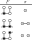
\includegraphics{flags-types-example}
    \caption{Example flags and their types}
    \label{fig:flags-types}
\end{figure}

We give the formal definitions:

\begin{definition}[Type]
    A \textbf{type} $\sigma$ of size $k$ is a graph with vertex set $[k]$. We write
    $|\sigma|$ to denote the size of the underlying graph. We write
    $\emptyset$ to denote the type consisting of the empty graph.
\end{definition}
\begin{definition}[$\sigma$-Embedding]
    Given a type $\sigma$ and a graph $F$, a \textbf{$\sigma$-embedding} is an injective
    function $\theta\colon[|\sigma|]\to V(F)$ which is a graph isomorphism between
    $\sigma$ and $F[\im \theta]$.
\end{definition}
\begin{definition}[$\sigma$-Flag]
    A \textbf{$\sigma$-flag} is a tuple $(F, \theta)$ where $\theta$ is an $\sigma$-embedding
    into $F$.
    If the embedding is implicit (e.g. if $\sigma=\emptyset$) we often drop the
    $\theta$ from the notation.
\end{definition}

\begin{note}
    A type $\sigma$ is implicitly itself a $\sigma$-flag when taken with the
    identity embedding $\id\colon [|\sigma|] \to [|\sigma|]$. We often use this fact
    implicitly.
\end{note}

We then say that two flags are isomorphic if there is a graph isomorphism between the underlying
graphs which preserves the labels.
\begin{definition}[Flag Isomorphism]
    $f\colon V(F) \to V(F')$ is a $\sigma$-flag isomorphism
    from $(F,\theta) \to (F', \theta')$ if it is graph isomorphism $F \to F'$ such that
    $f(\theta(i)) = \theta'(i)\ \forall\ i\in [|\sigma|].$ We can
    write $(F,\theta)\cong (F',\theta')$ if such an $f$ exists.
\end{definition}

Now that we have a definition for flags we can build on our induced density function from
the introduction.

\subsection{Induced Counts and Density}

In the introduction we defined the induced count $c(F; G)$ to be the number of
$U\subseteq V(F)$ such that $G[U] \cong F$. We need to adapt this notion now to handle
labelled vertices which must be preserved by the isomorphism. In particular if $G[U] \cong F$
then $U$ must contain the labelled vertices of $G$.

\begin{definition}[Induced Count]
    Fix two $\sigma$-flags $(F,\theta), (G,\eta).$ We define the induced count of $(F,\theta)$ in
    $(G,\eta)$ written $c((F,\theta); (G,\eta))$
    as the number of subsets $\im(\eta)\subseteq U\subseteq V(G)$ such that
    $(F,\theta) \cong (G[U], \eta)$.\footnote{Where we restrict the codomain of $\eta$ appropriately}
\end{definition}

We can extend this notion of counting how many copies of $F$ there are in $G$ to ask
how many tuples of disjoint copies of $F_1, \dots, F_t$ are there in $G$ (where
disjoint means vertex-disjoint apart from the fixed labelled vertices).

Precisely we define $c(F_1, \dots, F_t; G)$ to be the number of
$U_1, \dots, U_t\subseteq V(G)$ such that $\im\eta = U_i \cap U_j\ \forall\ i, j \in [t]$ where
$i\neq j$ and $(F_i, \theta_i) \cong (G[U_i], \eta)$ for all $i\in [t].$

Note that if $c(F_1, \dots, F_t; G) > 0$ we know that $G$ must be large enough to fit
disjoint copies of $F_1, \dots, F_t$ leading us to the following definition.

\begin{definition}[Fit]
    We say $\sigma$-flags $F_1, \dots, F_t$ \textbf{fit} in $\sigma$-flag $G$ if
    $|G|-|\sigma| \geq \sum_{i=1}^t |F_i|-|\sigma|$.
\end{definition}

\begin{example}
    Consider the type $\sigma=\vertex$, a single vertex. Any $\sigma$-flag $(G,\eta)$ is
    just a graph with a specific distinguished vertex (the unique labelled vertex).

    Consider then the $\sigma$-flag $F=\edgemarked$, an edge with a single labelled vertex.
    For any $G$ with distinguished vertex $v$, $c(\edgemarked; G) = \deg_G(v)$ as explained
    above.

    Similarly, $c(\edgemarked, \edgemarked; G) = \binom{\deg(v)}{2}.$ This is as
    we are counting how many distinct pairs of vertices $(a, b)$ are there in $G$ such that
    $G[\{a, v\}] \cong \edgemarked$ and $G[\{b, v\}] \cong \edgemarked$.
    In other words, how many distinct pairs of vertices are there connected to
    $v$, which is clearly $\binom{\deg(v)}{2}.$
\end{example}

Now we can define the induced density by normalising the induced count by the max
possible number of such non-overlapping $t$-tuples.

\begin{definition}[Induced Density]
    Given $\sigma$-flags $F_1, \dots, F_t$ and $G$ define the \textbf{induced density} of
    $F_1, \dots, F_t$ in $G$ as:
    \[
    p(F_1, \dots, F_t; G)
    := \frac{c(F_1, \dots, F_t; G)}{
    \binom{|G|-|\sigma|}{|F_1|-|\sigma|, \dots,|F_t|-|\sigma|, R}}
    \]
    where we use multinomial coefficient notation with
    $R=(|G|-|\sigma|)-\sum_{i=1}^t |F_i|-|\sigma|$.
\end{definition}

\begin{note}
    Again, as in the \hyperref[sec:motivating_example]{motivating example in the introduction},
    we can interpret $p(F_1, \dots, F_t; G)$ in a precise probabilistic way.
    $p(F_1, \dots, F_t; G)$ is exactly the probability that
    $(F_i, \theta_i) \cong (G[U_i], \eta)\ \forall\ i\in[t]$ where
    $U_1, \dots, U_t \subseteq V(G)$ is a uniformly random $t$-tuple of subsets such that
    $U_i \cap U_j = \im \eta\ \forall i, j \in [t], i \neq j$.
\end{note}

\subsection{Graph Classes}

Often, we want to limit our view to a subset of all possible graphs. For example, we
will want to consider only triangle-free graphs when proving Mantel's theorem (TODO REF).

We pick some class of graphs $\Gcl$. For Razborov's flag algebras we assume that
$\mathcal{G}$ is hereditary, meaning it is closed under taking induced subgraphs. This will change
when we introduce our new local framework.

Then for any type $\sigma$ we write $\Gcl^\sigma$ for the set of all $\sigma$-flags up to
isomorphism. We write $\Gcl^\sigma_n$ for the set of all $\sigma$-flags of size $n$.
We generally assume $\Gcl^\sigma$ is infinite for any type $\sigma\in\mathcal{G}$.
If $\sigma=\emptyset$ we often skip the superscript and just refer to
$\Gcl$ or $\Gcl_n$.

From this point all definitions and results are relative to some fixed graph class
$\mathcal{G}$.

Given some graph class $\mathcal{G}^\sigma$ then we get the very power \textit{chain rule}.
\begin{lemma}[The Chain Rule, Lemma 2.2 \cite{razborovFlagAlgebras2007}]
    \label{lemma:chain_rule}
    If $F_1, \dots, F_t \in \Gcl^\sigma$ are $\sigma$-flags which fit in $G\in\Gcl^\sigma$
    then for all $1 \leq s \leq t$ and every $n$ such that
    $F_1, \dots, F_s$ fit into a $\sigma$ flag of size $n$ and a
    $\sigma$-flag and $F_{s+1}, \dots, F_t$ fit in $G$ we have:
    \[
    p(F_1, \dots, F_t; G) = \sum_{F \in \mathcal{G}^\sigma_n}
    p(F_1, \dots, F_s; F)p(F, F_{s+1}, \dots, F_t; G).
    \]
\end{lemma}

This chain rule is one of the crucial properties that we will lose when we define our
local flags framework.

\subsection{The Algebra}

We've describe now our flags in detail, understanding a partially labelled flag and
the density functions they in some way represent. We would like to then formally
describe a structure on these flags such that relations in the structure describe true
relations about their associated density functions. As a start we want to be able
to describe linear combinations of flags, e.g. $\edge + \nonedge$ should in some
way represent $p(\edge; G) + p(\nonedge; G)$.

Take then the formal real vector space $\R\Gcl^\sigma$ for some fixed type $\sigma$,
this gives us a proper notion of these linear combinations of flags. We can then
linearly extend our density function $p$ to this space in the first argument giving
us a function $p\colon \R\Gcl^\sigma \times \Gcl^\sigma \to \R$ capturing that
$p(\edge + \nonedge; G) = p(\edge; G) + p(\nonedge; G) = 1$ and similar relations.

The chain rule (Lemma \ref{lemma:chain_rule}) tells us then that for any $F, G\in\Gcl^\sigma$
and $n \geq |F|$ we have $p(F; G) = \sum_{H \in \Gcl^\sigma_n}p(F; H)p(H; G)$. In
In particular, $p(F; H)$ is just some real number for each $H$ meaning
$p(F; G) - \sum_{H \in \Gcl^\sigma_n}p(F; H)p(H; G) = 0$ is a linear relation on
density functions which holds for all $F, G$. This tells us that in our algebra
any vector of the form $v = F - \sum_{H \in \Gcl^\sigma_n}p(F; H)H$ has the property
that $p(v; G) = 0$ for all $G\in\Gcl^\sigma$.

We can define the space $\mathcal{K}^\sigma$ as the span of vectors of the form
$F - \sum_{H \in \Gcl^\sigma_n}p(F; H)H$ for $F\in\Gcl^\sigma$, $n\geq |F|$ and
quotient out this relation from $\R\Gcl^\sigma$. Because $p(v; G) = 0$ for all
$v \in\mathcal{K}^\sigma, G \in\mathcal{G}$ our linear extension of $p$ is still well defined
on this space.

\begin{example}
    If $\Gcl$ is the class of triangle free graphs then we know from our
    \hyperref[sec:motivating_example]{motivating example} that
    $p(\edge; G) = \frac{2}{3}p(\triangletwoedge; G) + \frac{1}{3}p(\triangleoneedge; G)$
    for all $G\in\mathcal{G}$. We would like this to translate to a relation like
    $\edge = \frac{2}{3}\triangletwoedge + \frac{1}{3}\triangleoneedge$.

    In the space $\R\Gcl^\emptyset / \mathcal{K}^\emptyset$ both the vectors $\edge$ and
    $\frac{2}{3}\triangleoneedge + \frac{1}{3}\triangleoneedge$ belong to the same
    coset, so they are indeed equal. Hence this space does capture this relationship.
\end{example}

However, linear combinations are not powerful enough. We also want to be able to make
statements about products of densities. Ideally we would be able to define a
product on vectors $f, g \in \R\Gcl^\sigma / \mathcal{K}^\sigma$ such that for any $G\in\Gcl^\sigma$
we have $p(f \cdot g; G) = p(f; G)\cdot p(g; G)$. Unfortunately we don't achieve the
ideal relation, but we do get the result asymptotically which is enough:
$p(f\cdot g; G) = p(f; G) \cdot p(g; G) + o(1)$.

\begin{definition}[$\sigma$ Flag Algebra]
    For fixed type $\sigma$ define the following product $\Gcl^\sigma \times \Gcl^\sigma \to \R\Gcl^\sigma / \mathcal{K}^\sigma$
    on $\sigma$-flags $F, G\in\Gcl^\sigma$.
    \[
        F \cdot G := \sum_{H \in \Gcl^\sigma_\ell} p(F, G; H) \cdot H
    \]
    for any $\ell \geq |F|+|G|-|\sigma|$.
    Extend this product then bilinearly to the space
    $\R\Gcl^\sigma \times \R\Gcl^\sigma$. This then induces a bilinear map
    $\R\Gcl^\sigma / \mathcal{K}^\sigma \times \R\Gcl^\sigma / \mathcal{K}^\sigma \to \R\Gcl^\sigma / \mathcal{K}^\sigma$.

    This is all well defined due to Lemma 2.4 in \cite{razborovFlagAlgebras2007}.

    This turns the space
    $\R\Gcl^\sigma / \mathcal{K}^\sigma$ into an algebra. We call this the
    $\sigma$ flag algebra $\Acl^\sigma$.

\end{definition}

This algebra is then associative, commutative and unital
(also lemma 2.4 in \cite{razborovFlagAlgebras2007}).

Now we see the theorem which tells us why this product is useful:
\begin{theorem}[Theorem 2 \cite{silvaFlagAlgebrasFirst2016}]
    For fixed type $\sigma$, vectors $f, g\in \Acl^\sigma$ we have
    \[
        |p(f\cdot g; G) - p(f; G)\cdot p(g; G)| \in O\left(\frac{1}{|G|}\right)
    \]
    where $G\in\Gcl^\sigma$.
\end{theorem}

What this theorem tells us is that our symbolic product corresponds to a valid product of
the underlying density functions in the limit, which we can use to prove asymptotic results.

\begin{example}
    Returning to our example with $\sigma=\vertex$ and $F=\edgemarked$ we can compute that (choosing representative of cosets etc) we have
    $\edgemarked^2 = \trianglemarked + \triangletwoedgemarked.$ Let $G$ be a $\vertex$-flag
    with labelled vertex $v$. Then we know $c(\edgemarked; G) = \deg v$ from before.
    Then we can see that $c(\trianglemarked; G) + c(\triangletwoedgemarked)$ counts
    all possible ways of choosing pairs from the neighbourhood of $v$ hence
    $c(\trianglemarked; G) + c(\triangletwoedgemarked; G) = \binom{\deg v}{2}$.
    Therefore:
    \[
    \begin{split}
        p(\edgemarked; G)^2 - p(\edgemarked^2; G)
        &= \left(\frac{c(\edgemarked; G)}{|G|-1}\right)^2
            - p(\trianglemarked; G) - p(\triangletwoedgemarked; G)\\
        &= \left(\frac{\deg v}{|G|-1}\right)^2
            - \frac{c(\trianglemarked; G) + c(\triangletwoedgemarked; G)}{\binom{|G|-1}{2}}\\
        &= \left(\frac{\deg v}{|G|-1}\right)^2
            - \frac{\binom{\deg(v)}{2}}{\binom{|G|-1}{2}}\\
        &= \frac{\deg v}{(|G|-1)^2(|G|-2)}
            + \frac{\deg v}{(|G|-1)(|G|-2)}\\
        &= O\left(\frac{1}{|G|}\right).
    \end{split}
    \]
    as $\deg(v)\in O(|G|)$. Hence in the limit for large graphs $|G|$ we get
    the multiplicative relationships we're looking for. This will be made more precise
    in section TODO.
\end{example}


\chapter*{Popular summary}
\addcontentsline{toc}{chapter}{Popular summary}
Popular summary (half to one page, in English or Dutch, accessible to a first year bachelor student in mathematics)

\printbibliography{}

\end{document}
